% Numbers checked against results/aggregate/*.csv (Oct 16 2026). Build: make report
\documentclass[11pt]{article}

\usepackage[margin=1in]{geometry}
\usepackage{graphicx}
\usepackage{booktabs}
\usepackage{caption}
\usepackage[section]{placeins}
\usepackage{hyperref}

\graphicspath{{../results/aggregate/figures/}}

\title{Similar Patients, Shared Outcomes:\\
A Network Analysis of Patient Similarity and Information Leakage in EHRSHOT}
\author{Sanjay Malla \and Quade Leonard \and Ean Stedham}
\date{CIS 4930 / CAI 5155 Network Analysis and Machine Learning with Graphs\\
University of South Florida, Fall 2026\\[4pt]
October 2026}

\begin{document}
\maketitle

\begin{abstract}
We represent hospital records from Stanford's EHRSHOT dataset as networks in which each node is a hospital stay and two stays are connected when the patients' diagnosis histories are very similar. Using standard network measures, we ask whether connected stays share outcomes for two questions: will the stay last a week or more, and will the patient be newly diagnosed with high blood pressure within a year? We compare an \emph{honest} network, built only from diagnoses recorded before the moment of prediction, with a \emph{cheating} network that also uses later diagnoses, and with a randomly rewired network. Honest networks consist of many tight groups, and connected stays share outcomes far more often than chance. Adding future diagnoses barely changes this for hospital stays, but clearly strengthens it for high blood pressure, because the later record contains the very diagnosis being predicted. A second network, linking diagnoses that tend to follow one another, recovers recognisable families of conditions such as heart failure and sepsis.
\end{abstract}

\section{Introduction}

Hospitals record every diagnosis a patient receives in an electronic health record (EHR). One natural way to study these records is as a network. In our networks each node is a hospital stay, and an edge connects two stays whose diagnosis histories look alike. The idea is the same as a film recommender that connects people with similar viewing histories: if similar viewers liked a film, you might too, and if similar patients had a long hospital stay, this patient might too.

We ask two questions. First, \emph{are networks of similar patients organised around clinical outcomes, and what structure do they have?} Second, \emph{what changes if the network accidentally uses information from the future?} This second problem is called \emph{information leakage}. If a network is built from diagnoses recorded after the moment we are trying to predict, it can look informative only because it has already seen the answer. Leakage is a common and serious mistake in medical machine learning, because it makes methods look better on paper than they could be in a real hospital.

We answer both questions with classical network analysis and no machine learning, so that every result can be traced to a simple, transparent measure.

\section{Data}
\label{sec:data}

EHRSHOT is a de-identified EHR dataset released by Stanford together with a set of clinical prediction tasks~\cite{wornow2023ehrshot}. We use the course's trimmed version, stored in the OMOP format, a shared layout for organising visits, diagnoses, and other medical records~\cite{hripcsak2015ohdsi}. It covers 6,731 patients, 944,132 visits, and 2.57 million diagnosis records.

\subsection{Two prediction questions}

We study two EHRSHOT tasks. For each, the \emph{prediction time} is the moment the question is asked, and the \emph{label} is the true answer.
\begin{itemize}
  \item \textbf{Long stay.} At the end of the admission day, will this hospital stay last 7 days or more?
  \item \textbf{New high blood pressure.} At discharge, will the patient be diagnosed with essential hypertension for the first time within the next year? Stays of patients who already have the diagnosis are skipped.
\end{itemize}
The trimmed data do not include ready-made labels, so we rebuilt them from the EHRSHOT definitions. Where our labels and Stanford's official labels cover the same stays, they agree 99.84\% (long stay) and 99.40\% (high blood pressure) of the time. Table~\ref{tab:labels} summarises both questions.

\begin{table}[!htbp]
\centering
\caption{The two prediction questions.}
\label{tab:labels}
\begin{tabular}{lrrr}
\toprule
Question & Hospital stays & Patients & Positive \\
\midrule
Long stay ($\geq$ 7 days) & 6,998 & 3,844 & 25.4\% \\
New high blood pressure   & 3,511 & 2,217 & 12.8\% \\
\bottomrule
\end{tabular}
\end{table}

Each node in our patient networks is one hospital stay at its prediction time. A patient with several stays therefore appears as several nodes, which matters later because two stays of the same person tend to look alike.

\subsection{Two kinds of diagnosis codes}

Diagnoses are recorded as billing codes. In October 2015, US hospitals switched from the older ICD-9 billing codes to the newer ICD-10 codes (Figure~\ref{fig:codes}), so the same disease can have a different code depending on the year. The OMOP format also maps both versions to a single \emph{standardised diagnosis code} (from the SNOMED vocabulary). We use the standardised codes for all main analyses, so that a diagnosis made in 2014 and the same diagnosis made in 2017 count as the same thing. Section~\ref{sec:robust} shows what goes wrong otherwise.

\begin{figure}[!htbp]
\centering
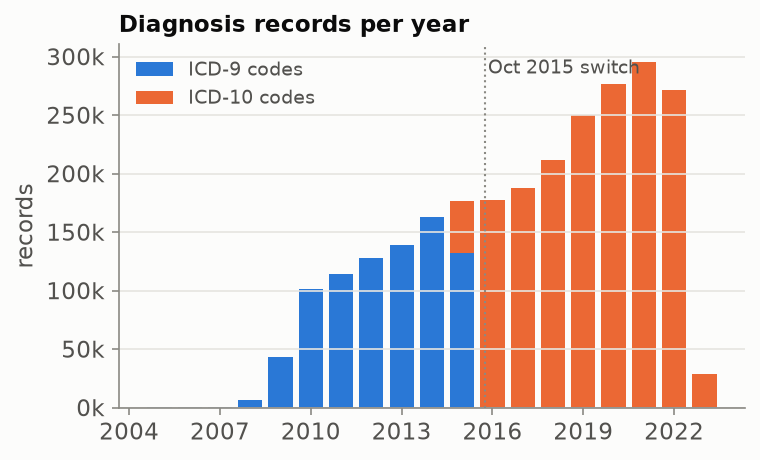
\includegraphics[width=0.7\textwidth]{01_billing_codes_by_year.png}
\caption{Diagnosis records per year. Hospitals switched from ICD-9 (blue) to ICD-10 (orange) billing codes in October 2015.}
\label{fig:codes}
\end{figure}

\section{Methods}
\label{sec:methods}

\paragraph{Building a network of stays.} For each stay we list which standardised diagnoses appear in the patient's record. We weight each diagnosis so that very common ones (which almost everyone has) count little and rare, specific ones count more; this is the TF-IDF weighting used in text search. Two stays are then compared with cosine similarity, which is 1 for identical diagnosis profiles and 0 for profiles with nothing in common. We connect two stays when each is among the other's 10 most similar stays.

\paragraph{Honest, cheating, and random networks.} For each question we build three networks with the same recipe:
\begin{itemize}
  \item \textbf{Honest:} only diagnoses recorded before the prediction time, which is all a real hospital could know.
  \item \textbf{Cheating:} the whole patient record, including diagnoses made after the prediction time. This deliberately introduces leakage. A cheating profile has about twice as many diagnoses as an honest one (97 against 48 on average for long stay).
  \item \textbf{Random:} the honest network with its connections randomly rearranged, while every stay keeps the same number of connections. We repeat this 10 times and report the average.
\end{itemize}
The random network tells us what to expect from the number of connections alone, so differences between the honest and random networks are structure that comes from the diagnoses.

\paragraph{What we measure.}
\begin{itemize}
  \item \textbf{Triangle rate} (transitivity): of all pairs of a stay's neighbours, the share that are also connected to each other.
  \item \textbf{Average path length}: the average number of steps between two stays in the largest connected group.
  \item \textbf{Communities}: groups of stays with many connections inside and few outside, found with the Leiden algorithm~\cite{traag2019louvain}, an improved version of Louvain~\cite{blondel2008fast}. \emph{Modularity} scores how clearly the groups are separated (above about 0.3 is clear).
  \item \textbf{Homophily}: whether connected stays share the same outcome more often than expected from how common each outcome is~\cite{lim2021large}. It is 0 when connections ignore the outcome and 1 when every connection joins stays with the same outcome.
  \item \textbf{Explained by communities}: the share of the variation in outcomes that is explained by which community a stay belongs to (0 means every community has the same outcome rate).
\end{itemize}

\paragraph{A network of diagnoses.} We also build a second kind of network, in which the nodes are the 200 most common diagnoses. We connect diagnosis A to diagnosis B when patients with A receive B within the following year more often than patients in general receive B. A connection is kept only if at least 10 patients show the pattern and it passes a strict significance test that accounts for the roughly 40,000 pairs tested. We then split this network into groups with the Girvan--Newman method~\cite{girvan2002community}, which repeatedly removes the connection that most acts as a bridge between groups, producing a tree of splits.

\section{Results}
\label{sec:results}

\subsection{Patient networks are made of many tight groups}

Table~\ref{tab:networks} gives the main measures and Figure~\ref{fig:pictures} shows the three long-stay networks. The honest networks are very different from random ones. Their triangle rate is about 0.5, against 0.001--0.002 in the random networks: patients with similar histories form tight triangles. Paths are longer than in the random networks (9.4 against 5.3 steps for long stay), because the network is a chain of local groups rather than one well-mixed whole. The community structure is very strong (modularity 0.94 and 0.92), with hundreds of small groups.

\begin{table}[!htbp]
\centering
\caption{Network measures for the honest, cheating, and random networks. Random values are averages over 10 rewirings.}
\label{tab:networks}
\small
\begin{tabular}{lrrrrrr}
\toprule
 & \multicolumn{3}{c}{Long stay} & \multicolumn{3}{c}{New high blood pressure} \\
\cmidrule(lr){2-4}\cmidrule(lr){5-7}
Measure & Honest & Cheating & Random & Honest & Cheating & Random \\
\midrule
Connections                 & 18,581 & 17,478 & 18,581 & 9,787 & 8,883 & 9,787 \\
Stays in largest group      & 88.2\% & 62.8\% & 95.6\% & 88.0\% & 74.6\% & 95.1\% \\
Triangle rate               & 0.494 & 0.660 & 0.001 & 0.479 & 0.589 & 0.002 \\
Average path (steps)        & 9.4 & 11.5 & 5.3 & 8.1 & 9.4 & 4.8 \\
Modularity                  & 0.938 & 0.977 & 0.546 & 0.922 & 0.958 & 0.540 \\
Homophily                   & 0.211 & 0.201 & 0.010 & 0.226 & 0.263 & 0.002 \\
Homophily, different patients & 0.239 & 0.228 & 0.010 & 0.115 & 0.154 & 0.002 \\
Same-patient connections    & 37.8\% & 39.3\% & 0.1\% & 29.5\% & 29.5\% & 0.2\% \\
Explained by communities & 0.109 & 0.130 & 0.008 & 0.074 & 0.136 & 0.010 \\
\bottomrule
\end{tabular}
\end{table}

\begin{figure}[!htbp]
\centering
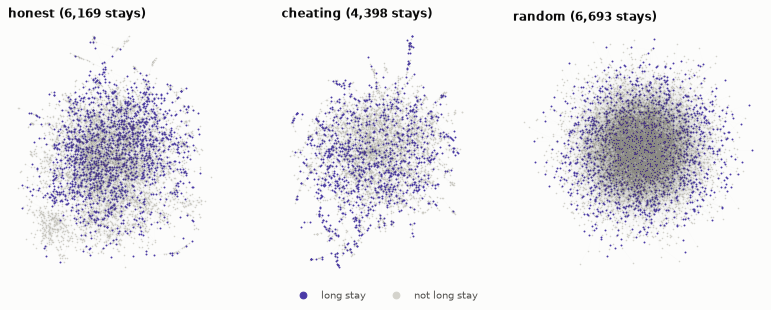
\includegraphics[width=\textwidth]{02_network_pictures.png}
\caption{The honest, cheating, and random long-stay networks (positions are for display only). Purple nodes are long stays. The honest and cheating networks break into many small, tight clusters; the random network is one tangled ball.}
\label{fig:pictures}
\end{figure}

\subsection{Connected stays share outcomes}

In both honest networks, connected stays share outcomes far more than chance: homophily is 0.21 for long stay and 0.23 for high blood pressure, against about 0.01 in the random networks. In plain numbers, 40\% of the connections of a long stay lead to another long stay, although only 25\% of all stays are long (24\% in the random network). For high blood pressure the figures are 32\% against a base rate of 13\%.

The communities show the same pattern (Figure~\ref{fig:groups}). Some communities have almost no long stays, while others have more than half, whereas in the random network every community stays close to the overall rate. Community membership explains about 11\% of the variation in long stay and 7\% in high blood pressure, against 1\% by chance.

\begin{figure}[!htbp]
\centering
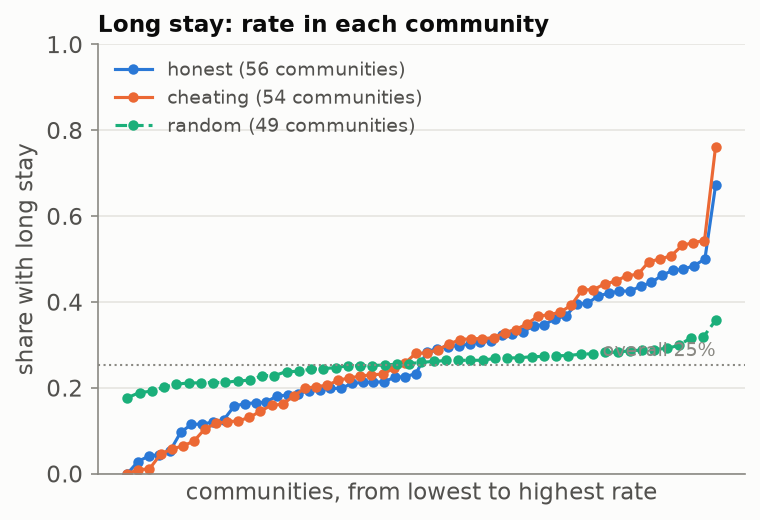
\includegraphics[width=0.49\textwidth]{02_group_outcome_rates.png}\hfill
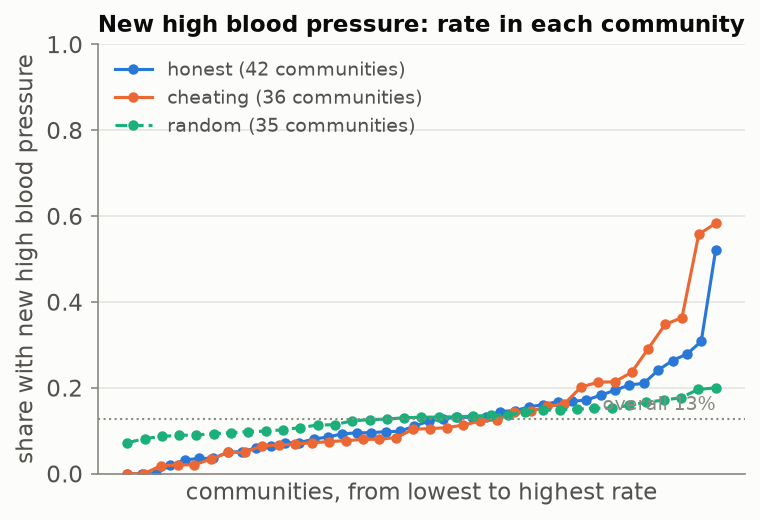
\includegraphics[width=0.49\textwidth]{03_group_outcome_rates.png}
\caption{Outcome rate in each community with at least 20 stays, sorted from lowest to highest. Left: long stay. Right: new high blood pressure. Honest and cheating communities range from almost no positives to well above the overall rate (dotted line); random communities all sit near it.}
\label{fig:groups}
\end{figure}

\paragraph{Connections between stays of the same patient.} About a third of the connections join two stays of the same patient (37.8\% for long stay, 29.5\% for high blood pressure). For long stay, these connections agree on the outcome 68.5\% of the time, close to the 62\% expected if outcomes were drawn at random, and removing them slightly \emph{raises} homophily (0.211 to 0.239). For high blood pressure they agree 94.9\% of the time against 77.7\% expected, and removing them halves homophily (0.226 to 0.115). So for long stay the pattern comes from different patients with similar histories, while for high blood pressure much of it comes from the same patient appearing several times.

\paragraph{Being central does not mean being sick.} How connected or central a stay is says almost nothing about its outcome: centrality scores separate positive from negative stays no better than a coin flip (AUROC 0.47--0.58).

\subsection{Leakage depends on the question}

Figure~\ref{fig:both} compares the honest and cheating networks for both questions.

For \textbf{long stay}, adding the future barely matters for outcomes. Homophily even drops slightly (0.211 to 0.201). The network's \emph{shape} does change: with twice as many diagnoses per stay, it breaks into more pieces (only 62.8\% of stays remain in the largest group). The strongest single giveaway in the future record is pleural effusion (fluid around the lungs), present for 63\% of long stays and 37\% of the others. That is a real difference, but it does not reorganise the network. The reason is simple: ``a stay of 7 days or more'' is not itself a diagnosis, so the future record does not contain the answer.

For \textbf{new high blood pressure}, leakage is clearly visible. Homophily rises from 0.226 to 0.263, and among connections between different patients it rises from 0.115 to 0.154, an increase of about a third. Community membership explains almost twice as much of the outcome (7.4\% to 13.6\%). Here the future record does contain the answer: by definition, every positive stay's later record includes the hypertension diagnosis, against only 13\% of negative stays (those diagnosed more than a year later). In the honest record, no single diagnosis differs by more than 11 percentage points between the two groups. This is a property of how the task is defined, not an early warning sign a hospital could use.

\begin{figure}[!htbp]
\centering
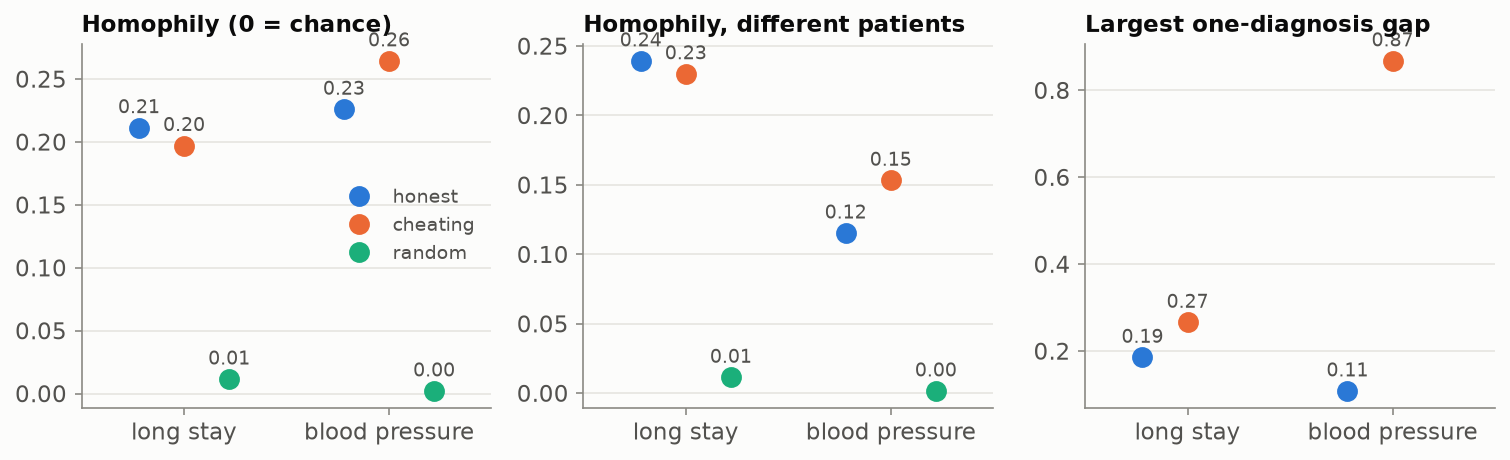
\includegraphics[width=\textwidth]{06_both_questions.png}
\caption{Honest (blue), cheating (orange), and random (green) networks for both questions. Left: homophily. Middle: homophily using only connections between different patients. Right: the largest difference between positive and negative stays in how often a single diagnosis appears. Cheating changes little for long stay but clearly helps for high blood pressure, where the diagnosis being predicted appears in the future record.}
\label{fig:both}
\end{figure}

Why does homophily rise only modestly when the answer is in the record? Because the weighting gives very little weight to diagnoses that many patients share, and hypertension is one of the most common diagnoses in the data. Figure~\ref{fig:cheat-htn} shows the effect connection by connection. This is a useful warning: leakage can be present and still look small in a single summary number.

\begin{figure}[!htbp]
\centering
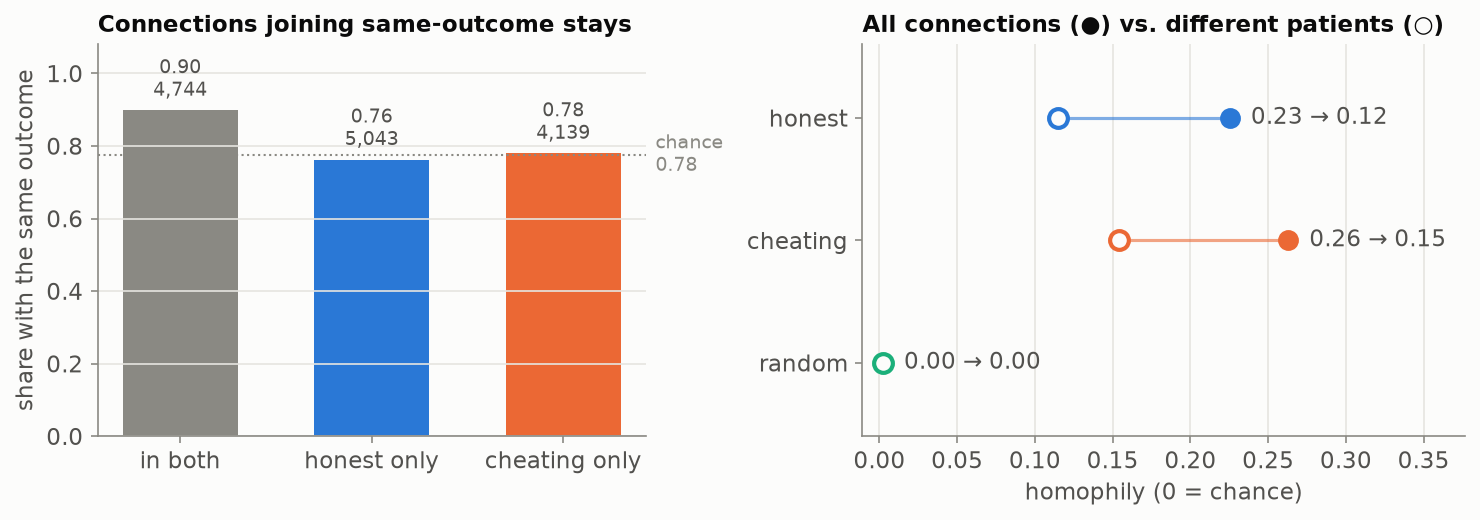
\includegraphics[width=0.9\textwidth]{03_what_cheating_changes.png}
\caption{New high blood pressure. Left: share of connections joining two stays with the same outcome, for connections found in both networks, only in the honest network, and only in the cheating network (dotted line: chance). Right: homophily with all connections (filled) and with only connections between different patients (open).}
\label{fig:cheat-htn}
\end{figure}

\subsection{Billing codes can split the data in two}
\label{sec:robust}

If we build the patient networks from raw billing codes instead of standardised codes, stays from before and after the 2015 switch almost never connect: only 1 of 18,693 long-stay connections and 5 of 9,892 high-blood-pressure connections cross the switch. (These billing-code networks have slightly different numbers of connections than the main ones.) With standardised codes, 3.0\% and 4.1\% of connections cross it. To check that the switch does not explain our outcome results, we shuffled outcomes separately among stays before and after 2015, which keeps any before/after difference but removes everything else. Homophily falls to 0.004 and 0.014, against 0.211 and 0.226 in reality, so the switch accounts for at most about 2\% and 6\% of the observed homophily. The leakage results also hold on billing codes: cheating raises high-blood-pressure homophily from 0.226 to 0.282 and leaves long stay unchanged (0.209 against 0.205).

\subsection{Diseases that follow each other form families}

The diagnosis network makes the billing-code problem even clearer. Built on raw billing codes, it has 134 diagnoses and 584 connections, but it falls apart into one piece of 69 codes, all ICD-10, and one of 47 codes, all ICD-9, with no connection between them (Figure~\ref{fig:rawtree}). Its first split separates old codes from new ones: it reflects a change in paperwork, not in medicine.

\begin{figure}[!htbp]
\centering
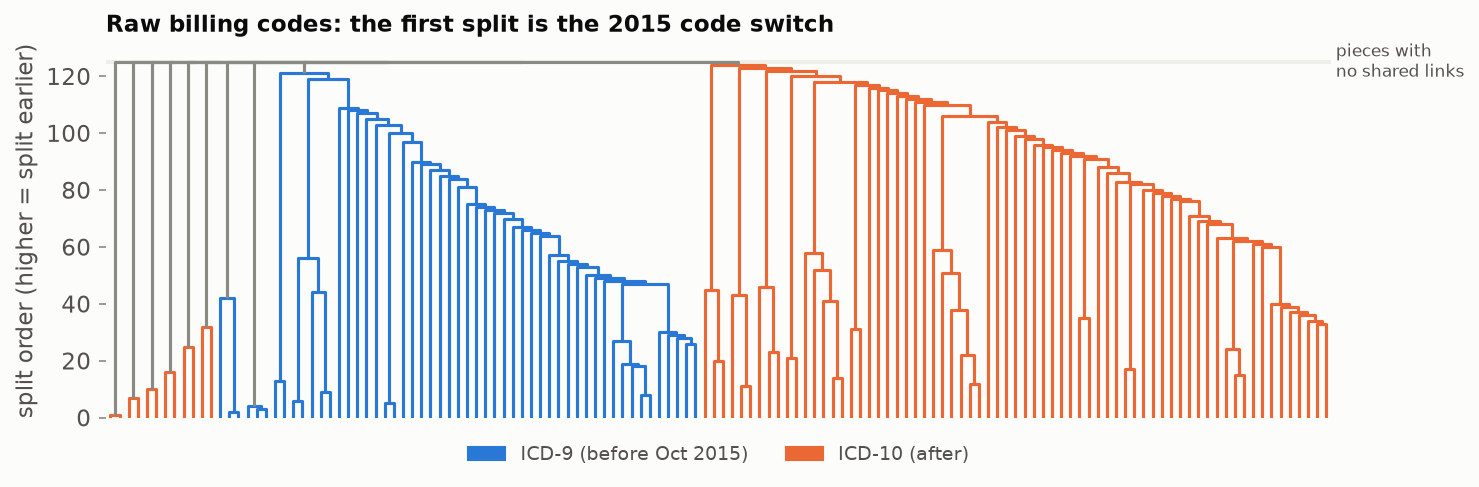
\includegraphics[width=0.75\textwidth]{04_raw_codes_tree.png}
\caption{Tree of splits for the diagnosis network built on raw billing codes. The top split separates ICD-9 from ICD-10 codes.}
\label{fig:rawtree}
\end{figure}

With standardised codes the network has 79 diagnoses and 142 connections, with one main piece of 60 diagnoses. The best cut of the Girvan--Newman tree gives 13 groups (modularity 0.57), similar to what Louvain finds (adjusted Rand index 0.65, where 1 means identical groups). The largest groups are clinically recognisable (Figure~\ref{fig:families}):
\begin{itemize}
  \item \textbf{Lung and breathing failure} (19 diagnoses): acute respiratory failure, pleural effusion, pneumonia, and collapsed lung tissue (atelectasis).
  \item \textbf{Sepsis and kidney failure} (18): sepsis, septic shock, bacteria in the blood, and acute kidney failure.
  \item \textbf{Heart failure} (14): congestive heart failure, cardiomyopathy, and heart disease caused by high blood pressure.
  \item Smaller groups: irregular heartbeat (5), pregnancy (4), and type 2 diabetes complications (4).
\end{itemize}
A few small pairs are the same condition recorded two ways, such as ``vomiting'' and ``nausea and vomiting''. These reflect recording habits rather than disease progression.

\begin{figure}[!htbp]
\centering
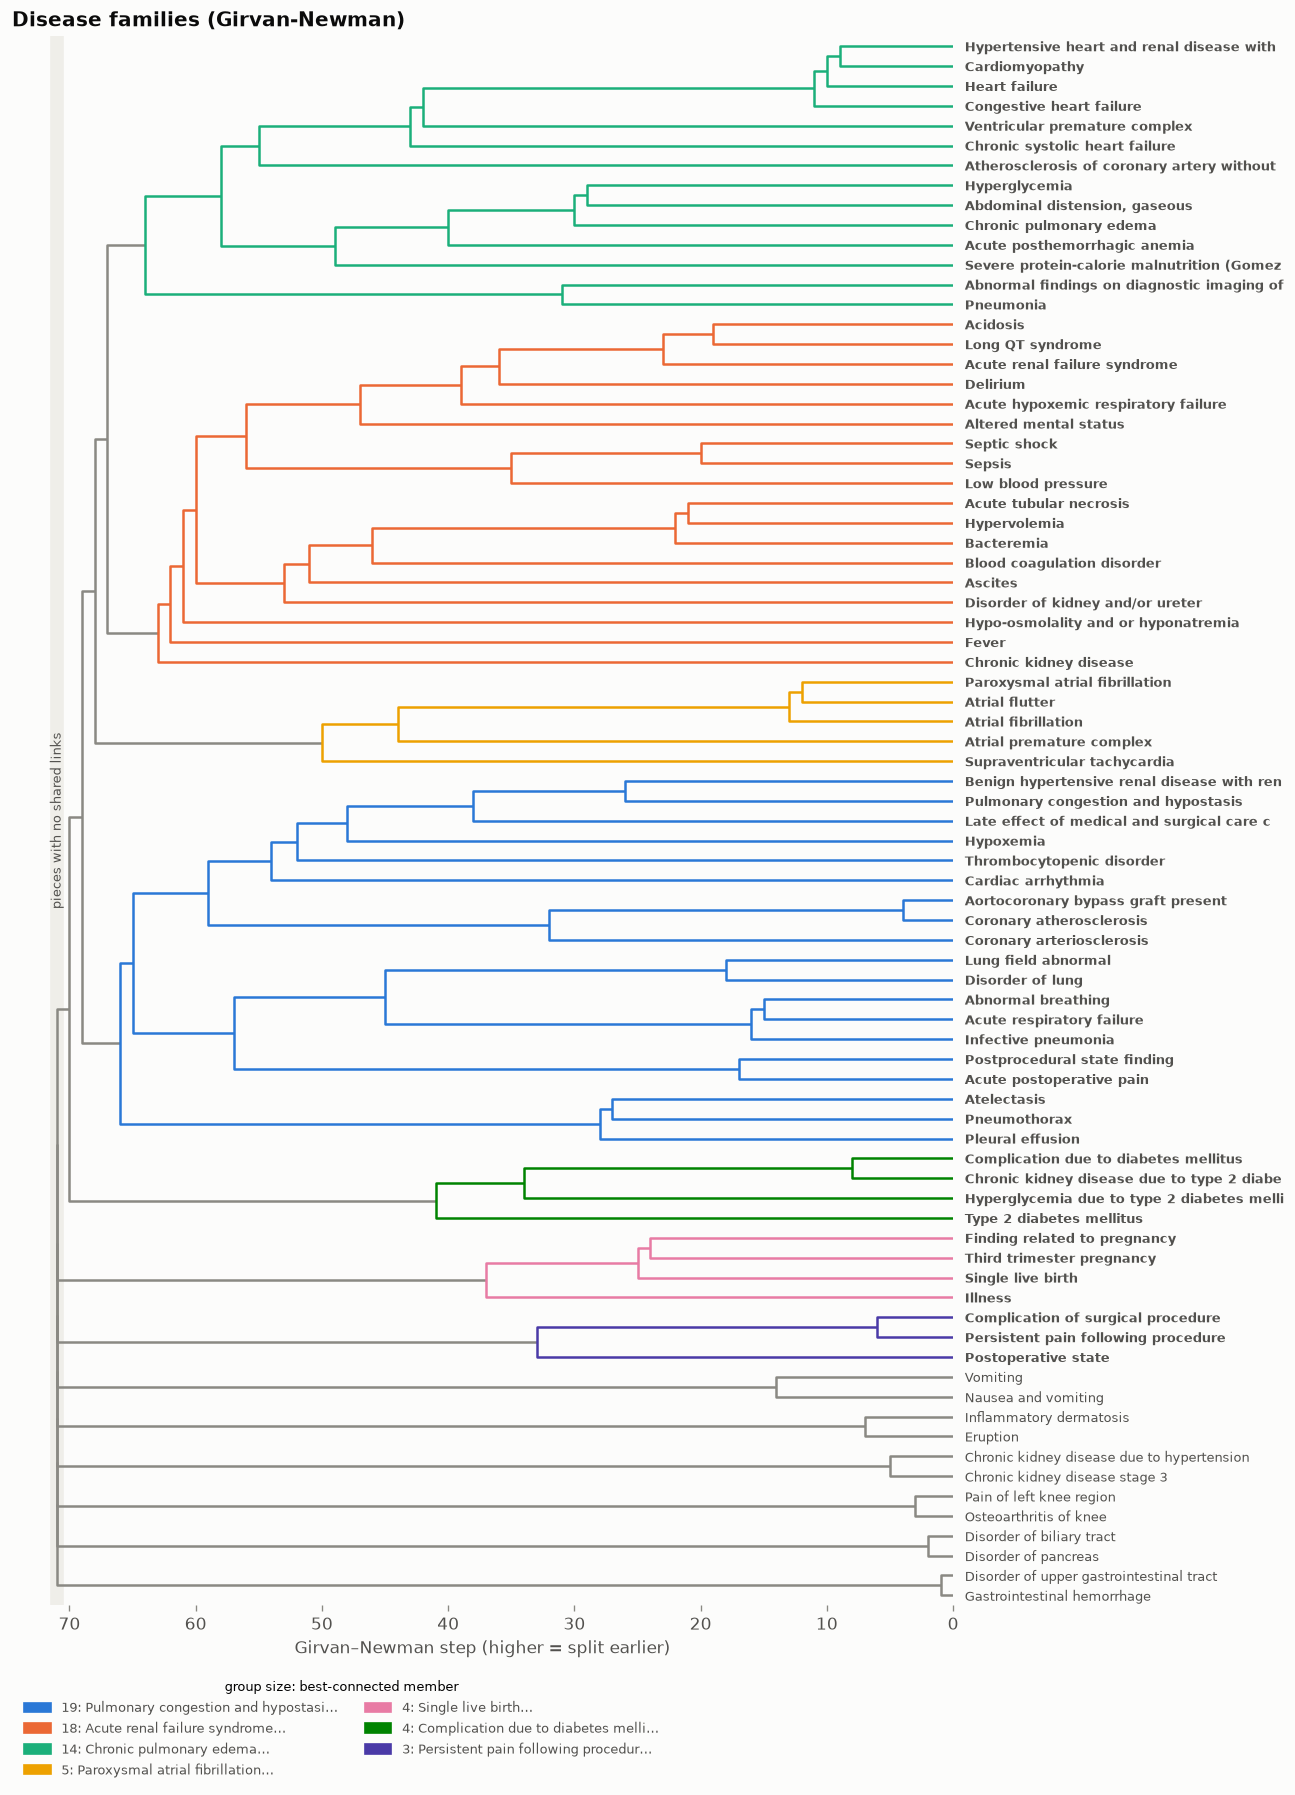
\includegraphics[width=\textwidth,height=0.55\textheight,keepaspectratio]{04_disease_families.png}
\caption{Tree of splits for the diagnosis network built on standardised codes, coloured by the 13 groups at the best cut. The large groups are lung and breathing failure, sepsis and kidney failure, and heart failure.}
\label{fig:families}
\end{figure}

\subsection{How things spread through the patient networks}

Finally, we simulate how a signal would travel through the patient networks. This is a mathematical analogy, not a model of real infection, and it shows how network shape affects the reach of information from one stay to its neighbours. In the SIR model~\cite{kermack1927contribution}, each stay is susceptible, ``infected'', or recovered. We start from 10 random stays; at each step an infected stay passes the signal to each neighbour with probability 0.3 and recovers with probability 0.1. After 10 steps the signal has reached 27\% of stays in the honest long-stay network, 13\% in the cheating network, and 87\% in the random network (47\%, 31\%, and 90\% for high blood pressure; Figure~\ref{fig:spread}, left). Tight groups and long paths slow the spread; the random network, with short paths and almost no triangles, lets it reach nearly everyone quickly.

The independent cascade~\cite{kempe2003maximizing} asks a more clinical question. We start from a random 5\% of the stays \emph{with} the outcome, and each newly reached stay gets one chance to pass the signal to each neighbour (probability 0.1). Of the stays reached in the honest network, 37\% are long stays (base rate 25\%) and 26\% are high-blood-pressure cases (base rate 13\%); in the random network the reached stays match the base rate (Figure~\ref{fig:spread}, right). Following connections from known cases therefore leads to other likely cases. This is the idea behind label propagation, a simple way to make predictions from a network.

\begin{figure}[!htbp]
\centering
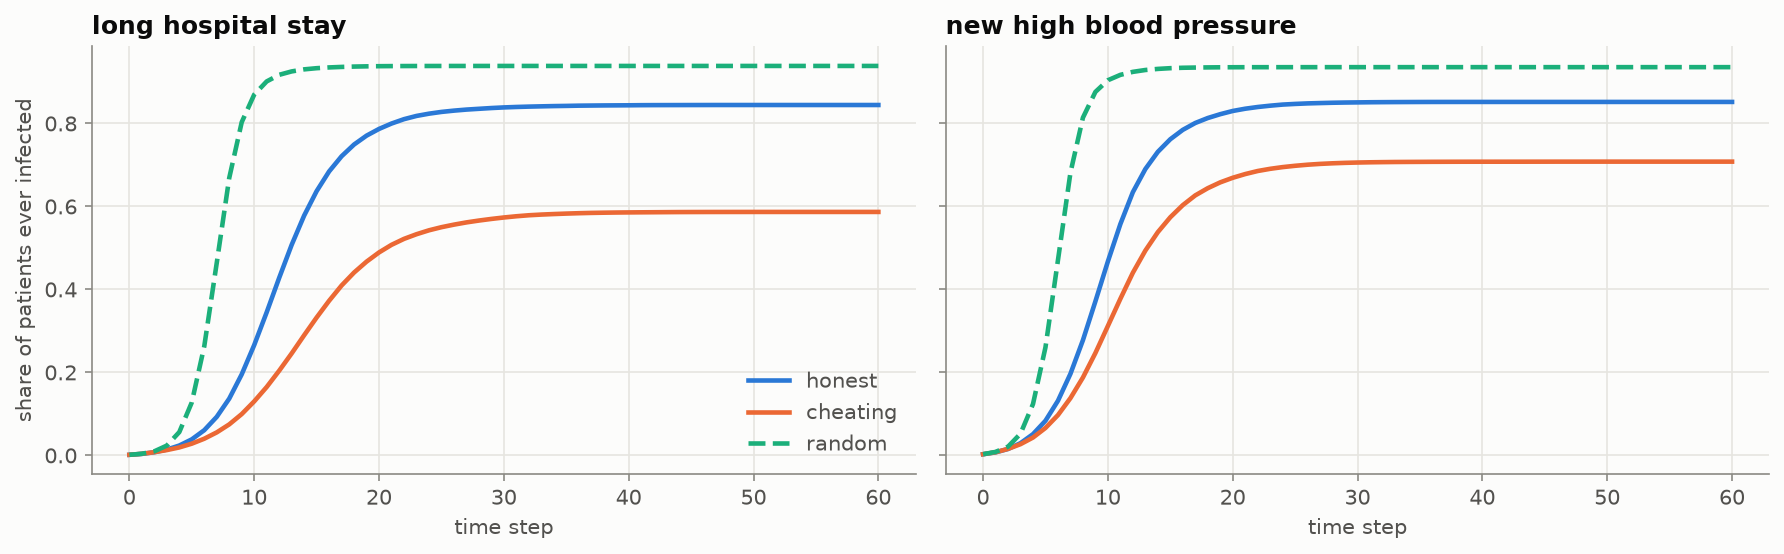
\includegraphics[width=0.49\textwidth]{05_sir_spreading.png}\hfill
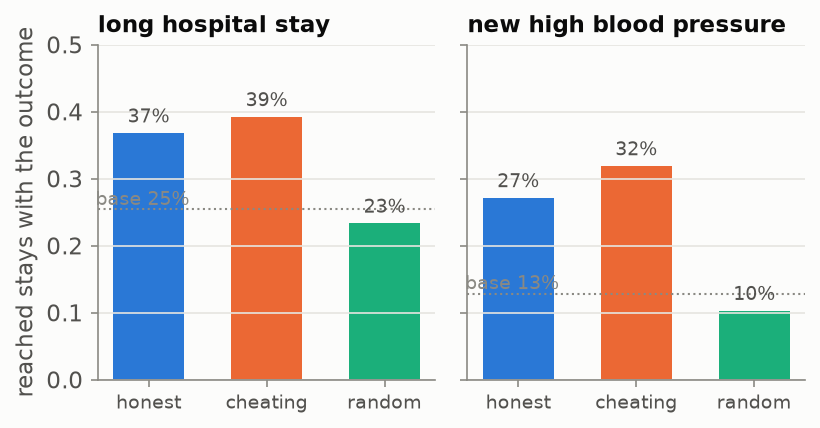
\includegraphics[width=0.49\textwidth]{05_cascade_reach.png}
\caption{Left: share of stays ever reached in the SIR simulation over time (average of 20 runs). Right: share of stays reached by a cascade from positive stays that are themselves positive, against the base rate (dotted line).}
\label{fig:spread}
\end{figure}

We also tried spectral partitioning~\cite{vonluxburg2007tutorial}, another way to split a network into groups. With 10 groups it finds much weaker structure than Leiden (modularity 0.41 against 0.93), but with as many groups as Leiden finds it nearly catches up (0.89). These networks have dozens of natural communities, not a few large ones.

\section{Discussion}
\label{sec:discussion}

Honest patient networks, built only from what was known at the time, are organised around clinical outcomes well beyond chance. They are highly clustered, split into strong communities, and those communities differ sharply in their outcome rates. Leakage behaves very differently for the two questions. For long stay, the outcome is a length of time rather than a diagnosis, so the future record adds detail but not the answer. For new high blood pressure, the future record contains the diagnosis itself, and the cheating network becomes more aligned with the outcome. Even then the effect looks modest in summary numbers, a reminder that leakage can hide inside small changes.

Simple network measures also revealed three problems in the data before any model was trained: the 2015 billing-code switch, which splits both kinds of networks when raw codes are used; connections between stays of the same patient, which carry much of the high-blood-pressure signal; and some official high-blood-pressure cases whose patients already had the diagnosis. Each of these could quietly inflate the results of a prediction model.

The diagnosis families agree with medical knowledge: breathing failure groups with pneumonia and pleural effusion, sepsis with kidney failure, and heart failure with cardiomyopathy. Pleural effusion, the strongest long-stay giveaway in the future record, belongs to the breathing-failure family, consistent with long stays being driven by serious lung and heart illness.

This study has several limitations. It describes patterns and does not test predictions on new patients. We use one way of building the networks (diagnoses only, 10 nearest neighbours), and adding medications or lab tests, or changing the number of neighbours, could change the picture. Homophily is computed with all outcomes known, which is fine for description but would itself be leakage in a prediction setting. Our rebuilt labels differ slightly from Stanford's official ones. Finally, a connection in the diagnosis network means two diagnoses tend to occur within a year of each other, not that one causes the other, and our grouping ignores which diagnosis came first.

\section{Conclusion and Future Work}
\label{sec:conclusion}

Networks of similar patients built from EHRSHOT carry real outcome structure: stays that look alike in their history tend to share outcomes, and the network's communities differ widely in outcome rates. Whether information from the future distorts these networks depends on whether the outcome itself appears in the future record. It does for a new diagnosis such as high blood pressure, and it does not for length of stay. Along the way, simple network measures exposed data problems early, before they could affect a model.

Our next step is to test whether honest patient networks actually improve predictions when only a handful of labelled examples are available, the \emph{few-shot} setting of the EHRSHOT benchmark~\cite{wornow2023ehrshot}. We will compare graph neural networks and label propagation on the honest networks against methods that ignore the network, use the cheating networks only as a leakage check, and handle connections between stays of the same patient explicitly.

\paragraph{Code and reproducibility.}\sloppy\ All code, analysis notebooks, and summary results are available at
\begin{center}\url{https://github.com/patient-graph-lab/ehrshot-patient-graphs}\end{center} To reproduce the analysis, install the Python environment with \texttt{uv sync}, place the course's EHRSHOT tables in \texttt{data/omop/}, and run the six notebooks in order. Alternatively, \texttt{make docker-check} runs everything in a clean container and confirms that the results in this report are reproduced. Patient-level data never leave our own machines, as required by the dataset's terms of use.

\bibliographystyle{plain}
\bibliography{references}

\end{document}
